\documentclass[11pt,letterpaper]{article}

\usepackage{graphicx}
\usepackage[margin=1in]{geometry}
\usepackage{amsmath}
\usepackage[T1]{fontenc}
\usepackage[utf8]{inputenc}
\usepackage{authblk}
\usepackage{fancyhdr}
\usepackage{lastpage}
\usepackage[parfill]{parskip}
\usepackage{subcaption}

\pagestyle{fancyplain}

% Headers
\lhead{}
\chead{}
\rhead{}

% Footers
\lfoot{}
\cfoot{}
\rfoot{\footnotesize Page \thepage\ of \pageref{LastPage}}

\renewcommand{\headrulewidth}{0.0pt} % No header rule
\renewcommand{\footrulewidth}{0.4pt} % Thin footer rule

\title{Federated Consistency Simulation: \\
 Increasing Likelihood of Conflicts Across Many Objects}
\date{August 10, 2016}
\author[ ]{Benjamin Bengfort}
\author[ ]{Pete Keleher}
\affil[ ]{Department of Computer Science}
\affil[ ]{University of Maryland}
\affil[ ]{\textit{\{bengfort,keleher\}@cs.umd.edu}}

\begin{document}

\maketitle

This report presents results that compare the Eventual, Raft, and Federated consistency models in our user-centric network against increasing probability of conflict ($P_c$). $P_c$ is a scale between 0 and 1 where $P_c = 0.0$ means that all replicas write to their own namespace with no overlap and $P_c = 1.0$ means that the namespace is complete shared by all replica servers. Any value in between indicates a varying level of overlap between the overlap of a replica's namespace.

Simulations were executed with 11 different access traces that implemented $P_c$ from 0.0 to 1.0 in 0.1 steps. All three simulations used the same access trace for each $P_c$ for a total of 33 simulations run. Details of the traces are shown in Table \ref{table:traces}. The trace also maintained a constant average of 30 names per device, 2,401 accesses per device, and 80 accesses per name.

\begin{table}[!h]
\centering
\begin{tabular}{ | c | c | c | c |}

    \hline
    $P_c$ & Accesses & Namespace & Avg. Devices per Name \\
    \hline
    0.0 & 48,021 & 600 &  1 \\
    0.1 & 48,021 & 278 &  2 \\
    0.2 & 48,022 & 165 &  3 \\
    0.3 & 48,026 & 121 &  4 \\
    0.4 & 48,027 & 91  &  6 \\
    0.5 & 48,031 & 71  &  8 \\
    0.6 & 48,033 & 62  &  9 \\
    0.7 & 48,037 & 53  & 11 \\
    0.8 & 48,035 & 42  & 14 \\
    0.9 & 48,034 & 36  & 16 \\
    1.0 & 48,038 & 30  & 20 \\
    \hline

\end{tabular}

\caption{\textsf{Change in the number of names and amount of overlap with increasing $P_c$}}
\label{table:traces}
\end{table}

The simulation kept all other parameters fairly pessimistic in order to complete the run as quickly as possible. The local area latencies were normally distributed such that $\lambda_{\mu}=30, \lambda_{\sigma}=5$ and the wide area latencies were distributed as $\lambda_{\mu}=1000, \lambda_{\sigma}=20$. Using the Bailis model, the tick parameter, $T = 10000$ so that the election timeout was uniformly selected in the range $[10000, 20000]$, the heartbeat interval was 5000 and the anti-entropy delay 2500. Accesses were triggered with a delay between accesses normally distributed such that $A_{\mu}=1800, A_{\sigma}=240$ with a read probability, $P_r=0.58$.

\begin{figure}[!h]
    \centering
        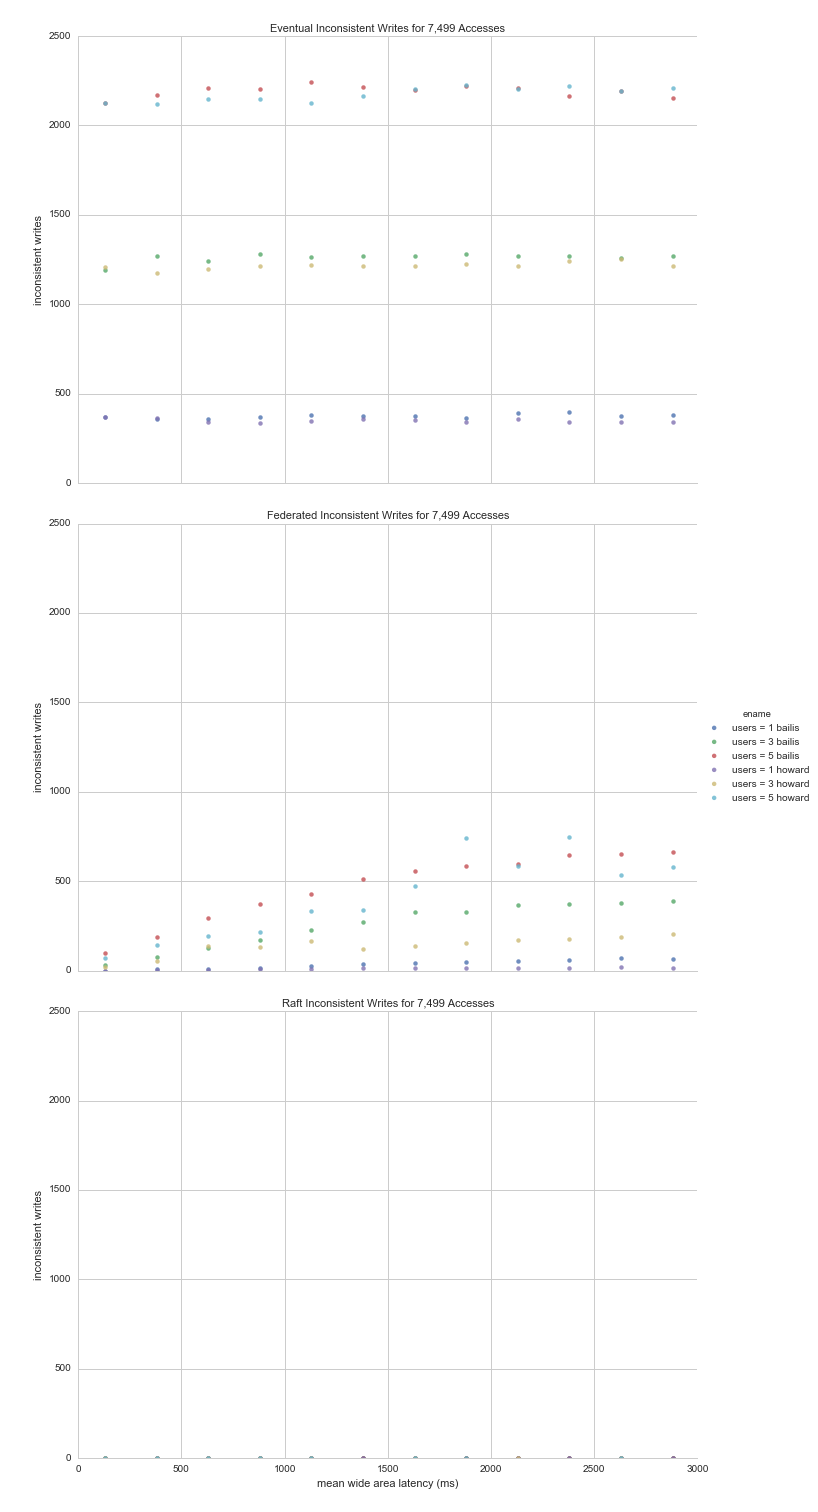
\includegraphics[width=\textwidth]{figures/inconsistent_writes.png}
        \caption{\textsf{Raft does not allow inconsistent writes by rejecting any (dropping them) that are remotely written. As the conflict increases, the number of inconsistent writes increases for both Federated and Eventual, but the Raft core in Federated minimizes the effect of increasing conflict. Note that there are no inconsistencies in any system given zero conflict.}}
        \label{fig:inconsistent_writes}
\end{figure}

\begin{figure}[!h]
    \centering
        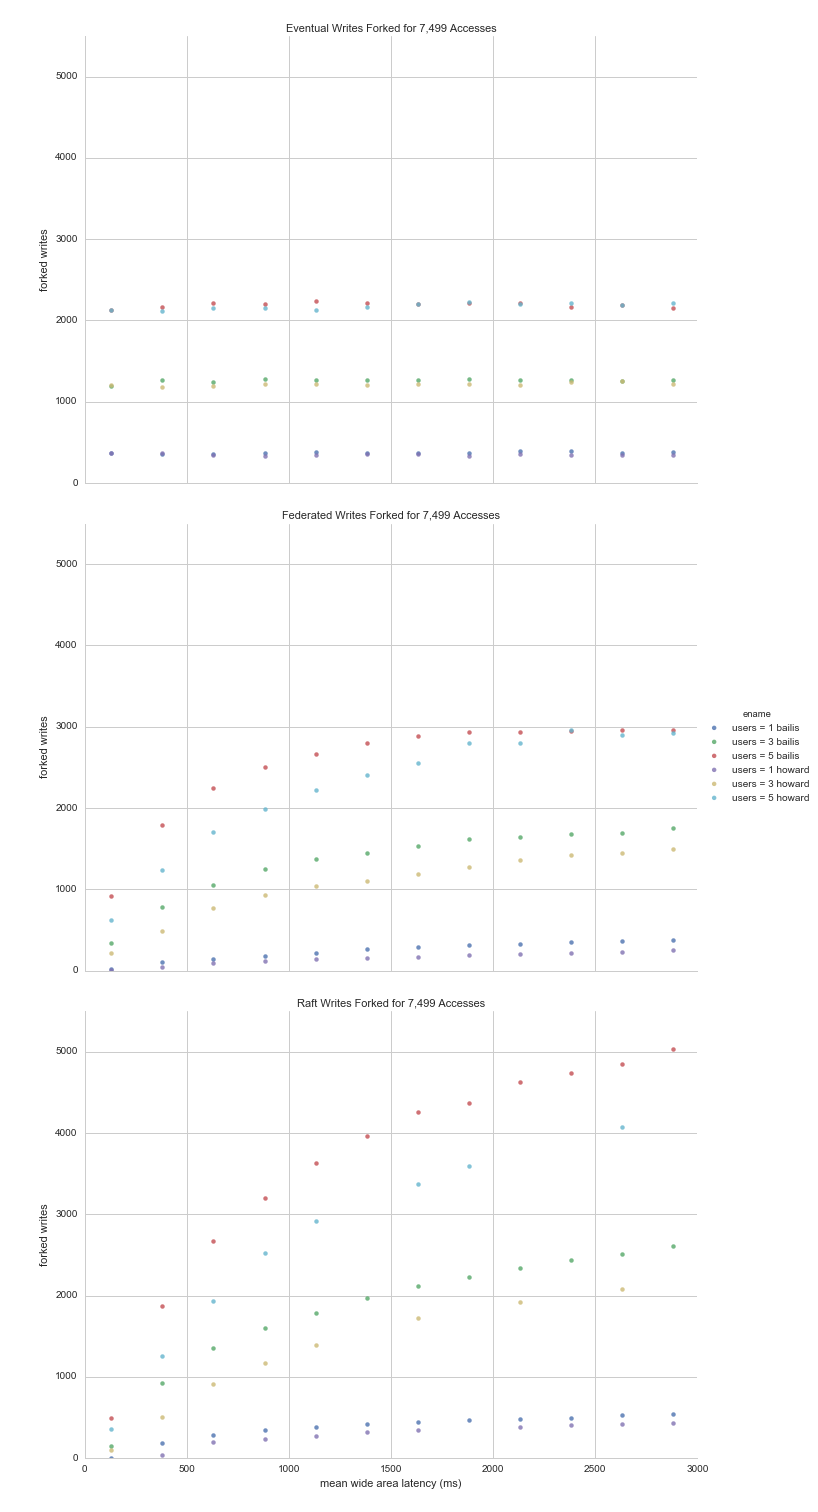
\includegraphics[width=\textwidth]{figures/forked_writes.png}
        \caption{\textsf{This figure is a contrast to \ref{fig:inconsistent_writes} to show how many inconsistencies are being generated. Raft now does have forks, because this figure excludes those that Raft would normally reject. As expected, forks increase as the conflict increases. What was not expected is that at even zero conflict, both Federated and Eventual have forks occurring (though in the previous figure, all three have zero inconsistencies at zero conflict). This may be due to the difficulty in counting forks I mentioned in an earlier discussion, but I will look into it.}}
        \label{fig:forked_writes}
\end{figure}


\begin{figure}[!h]
    \centering
        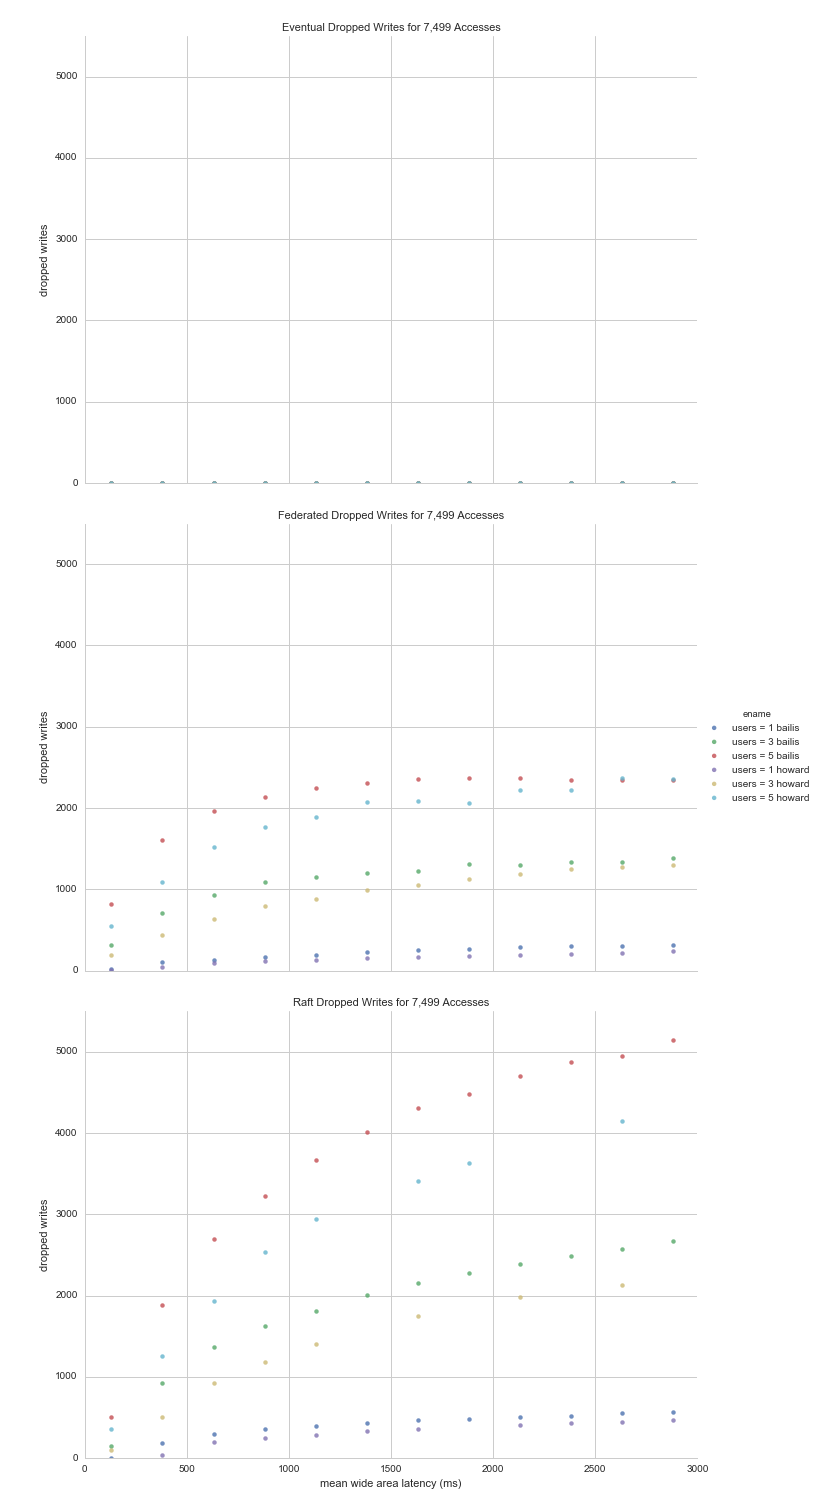
\includegraphics[width=\textwidth]{figures/dropped_writes.png}
        \caption{\textsf{This graph is the inverse of \ref{fig:forked_writes} showing that Eventual does not drop any writes or block progress, whereas both Raft and Federated must reject writes in order to maintain the client-consistency guarantee. Federated once again seems to do better than even at balancing Eventual and Raft. }}
        \label{fig:dropped_writes}
\end{figure}

\begin{figure}[!h]
    \centering
        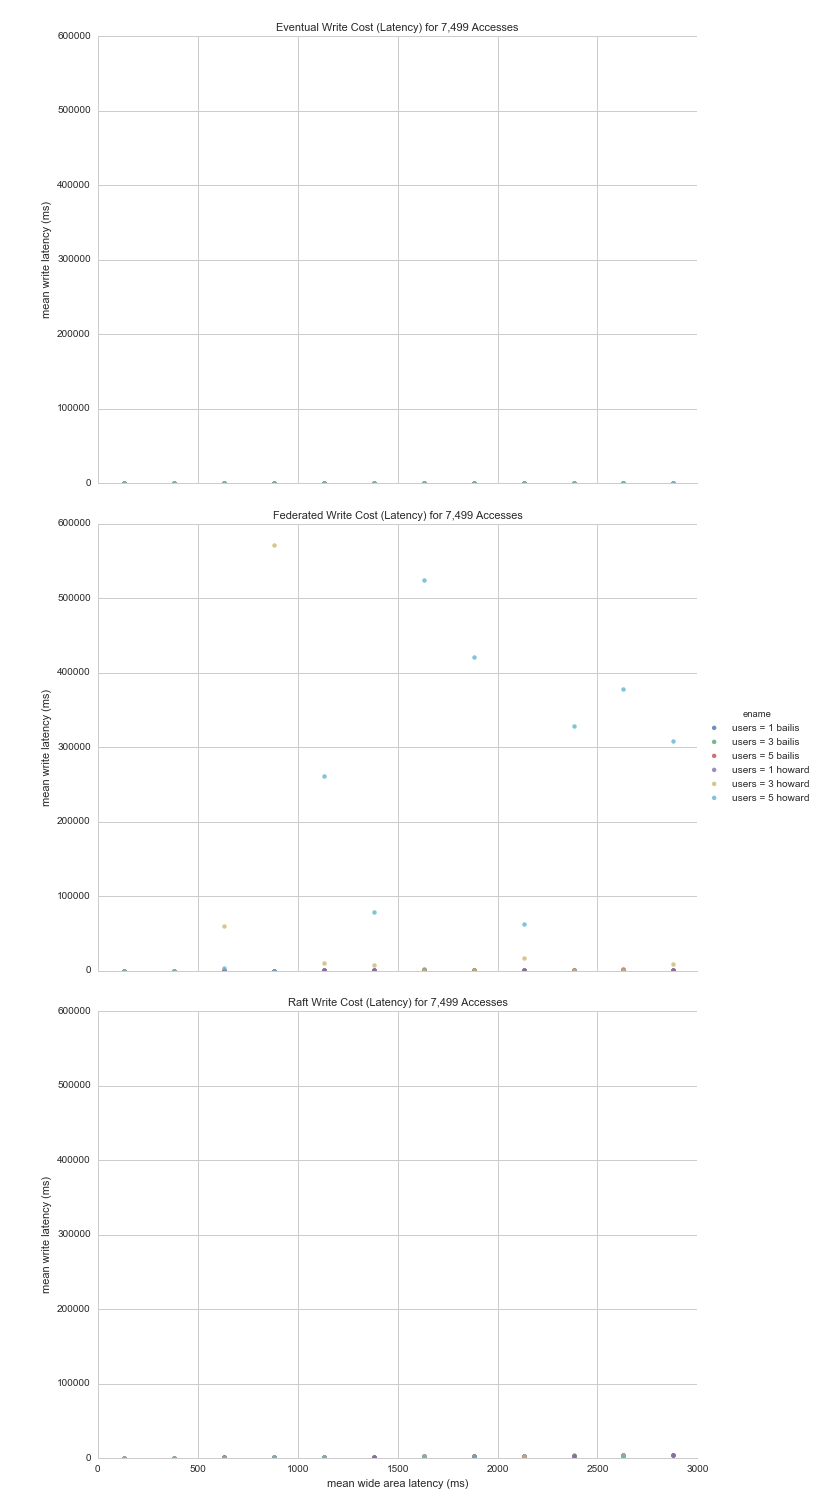
\includegraphics[width=\textwidth]{figures/write_latency.png}
        \caption{\textsf{The cost of a write is directly related to the cost of a remote write to the leader and a broadcast across the wide area in Raft, whereas writes are instantaneous in eventual since they write to a local cache. Federated averages the cost of progress according to how many nodes are participating in which scheme. I'm not sure what the blip is where the $P_c=0.6$, I assume it's an imbalance in the writes to the Raft nodes vs. writes to the eventual nodes.}}
        \label{fig:write_latency}
\end{figure}


\begin{figure}[!h]
    \centering
        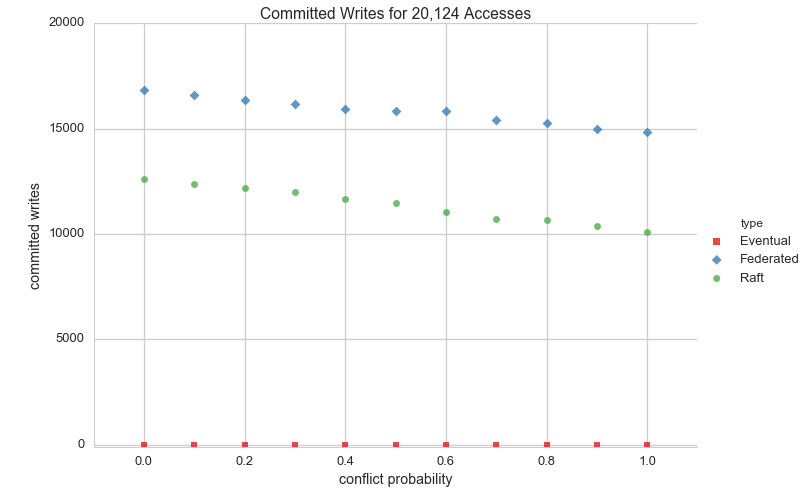
\includegraphics[width=\textwidth]{figures/committed_writes.png}
        \caption{\textsf{Eventual has no notion of committing writes, Raft should commit every write unless it has to drop due to a conflict. Federated is able to get more commits because there are less dropped writes.}}
        \label{fig:committed_writes}
\end{figure}

\begin{figure}[!h]
    \centering
        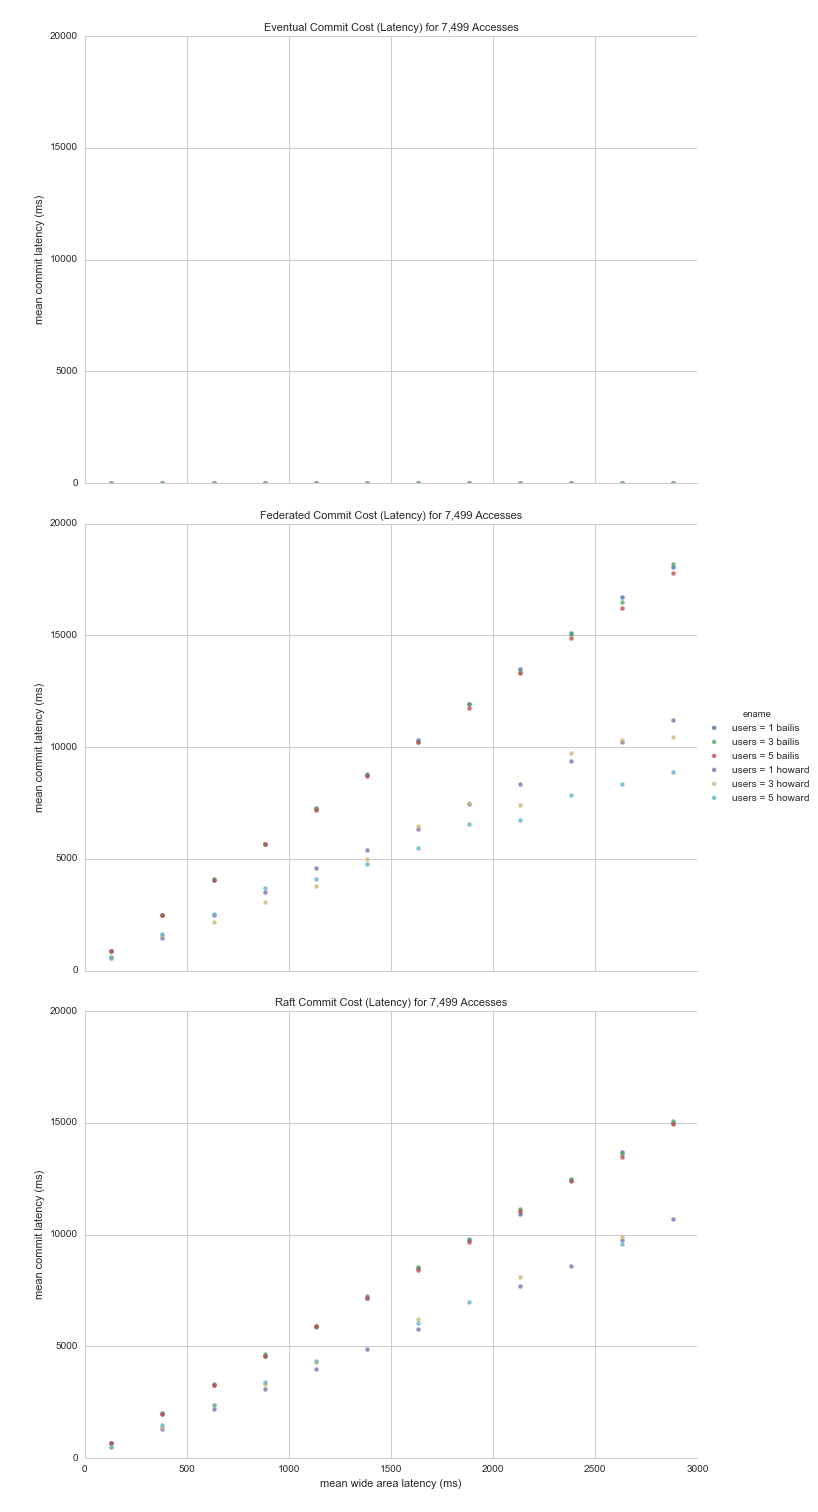
\includegraphics[width=\textwidth]{figures/commit_latency.png}
        \caption{\textsf{Even though Federated commits more writes, it does take Federated longer to commit a write because it has to include the anti-entropy delay before the write reaches a Raft node in the commit latency.}}
        \label{fig:commit_latency}
\end{figure}

\begin{figure}[!h]
    \centering
        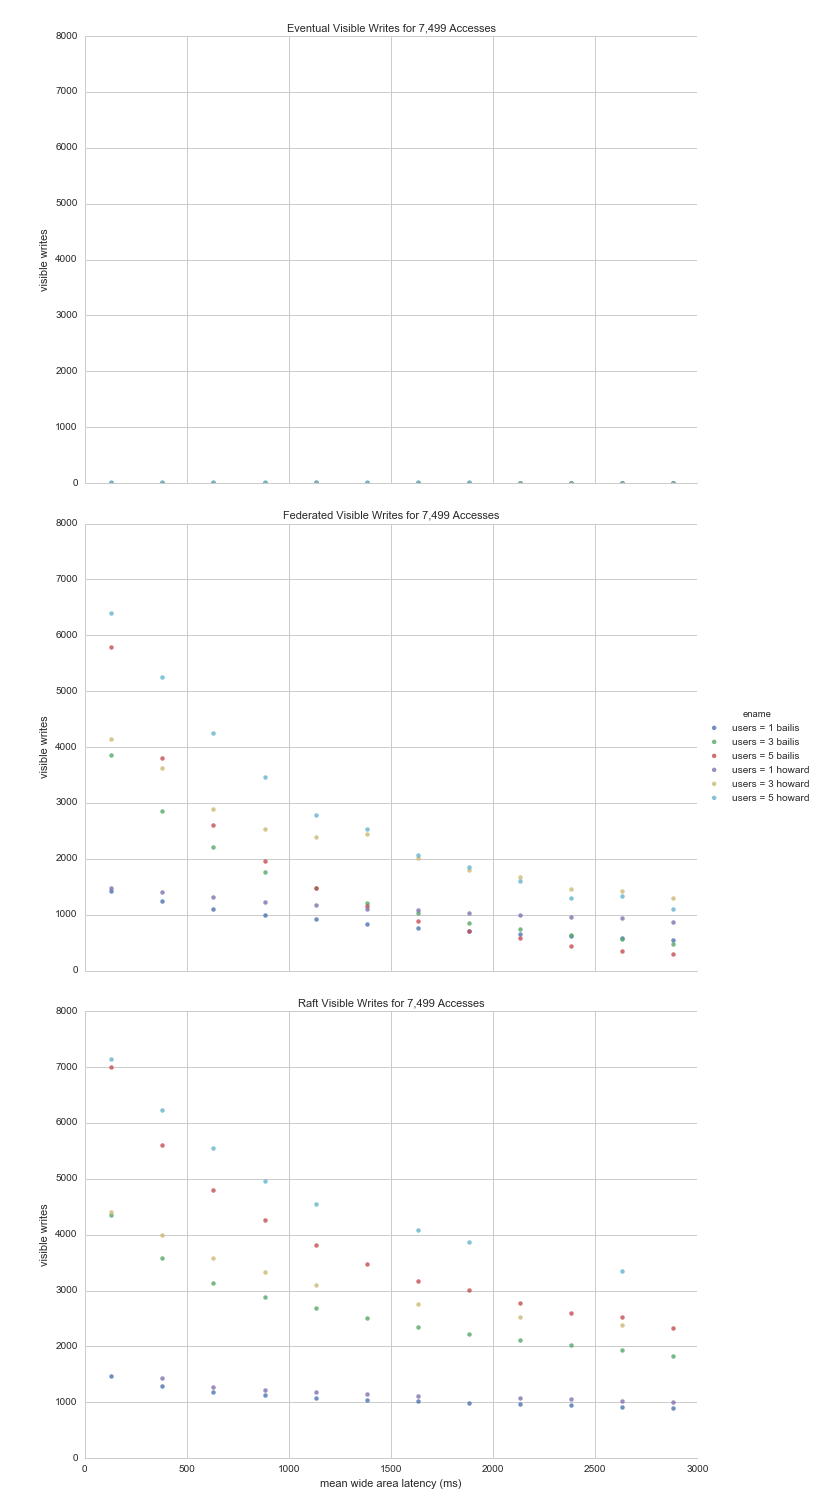
\includegraphics[width=\textwidth]{figures/visible_writes.png}
        \caption{\textsf{There is currently a bug with Eventual that is causing writes to not become fully replicated on a few nodes, but those numbers aren't zero -- they're just in the 10s of fully visible writes. Raft uses a broadcast mechanism, so all writes become fully visible unless they are dropped. Federated on the other hand, suffers from Eventual writes getting stomped on, and so as conflict increases, the number of fully visible writes goes down; though this will also be fixed with the Eventual bug fix.}}
        \label{fig:visible_writes}
\end{figure}

\begin{figure}[!h]
    \centering
        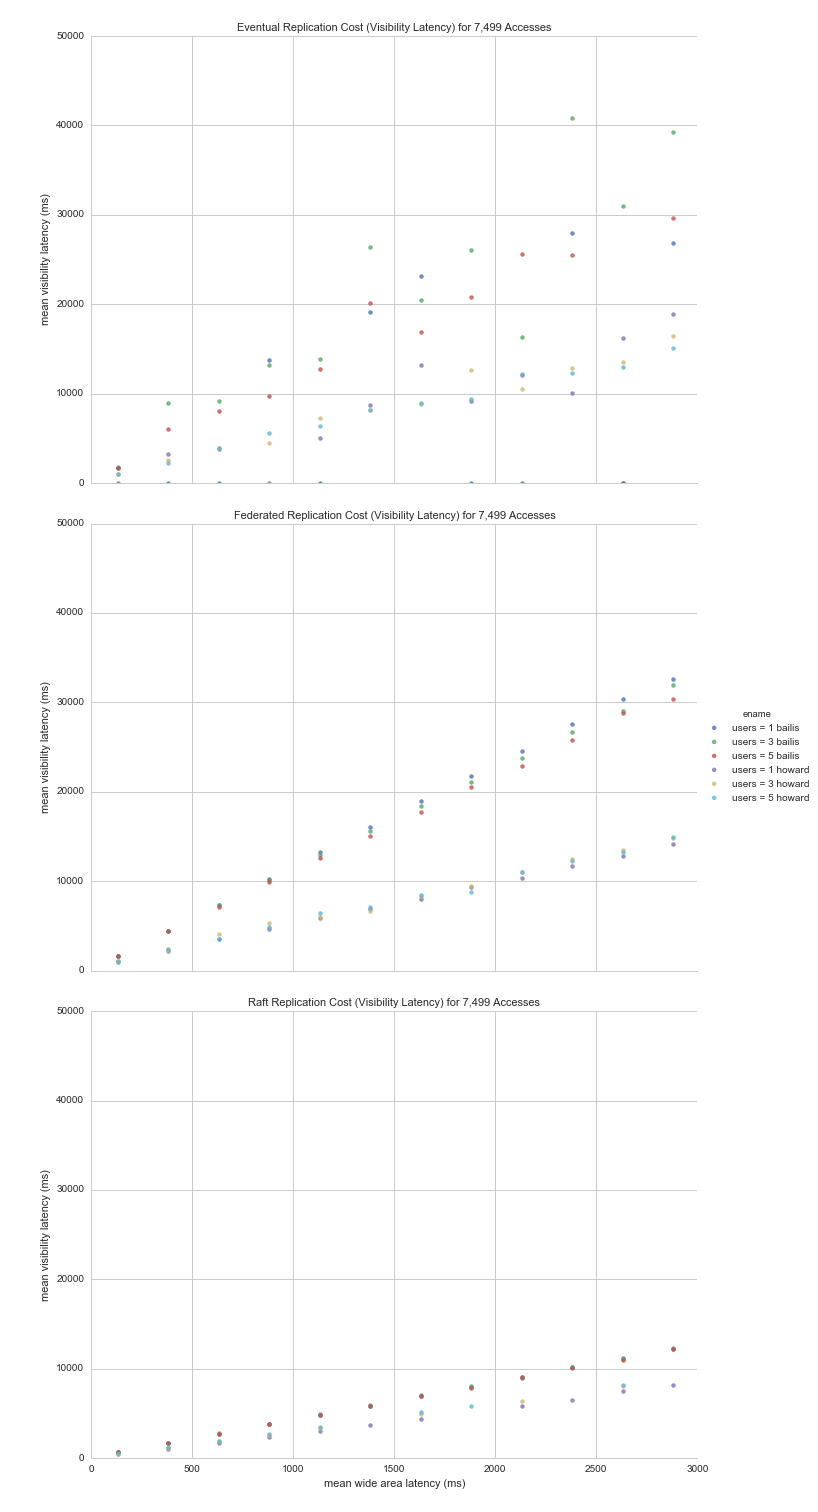
\includegraphics[width=\textwidth]{figures/visibility_latency.png}
        \caption{\textsf{Once the Eventual visibility bug is fixed we should see that it takes much longer to make eventual writes become visible because of the anti-entropy mechanism; convergence delay will define how long it takes a write to become fully visible. Federated does not do as well as Raft because it also has anti-entropy delays, but does improve on Eventual since it has a core that broadcasts writes across the wide area.}}
        \label{fig:visibility_latency}
\end{figure}

\begin{figure}[!h]
    \centering
        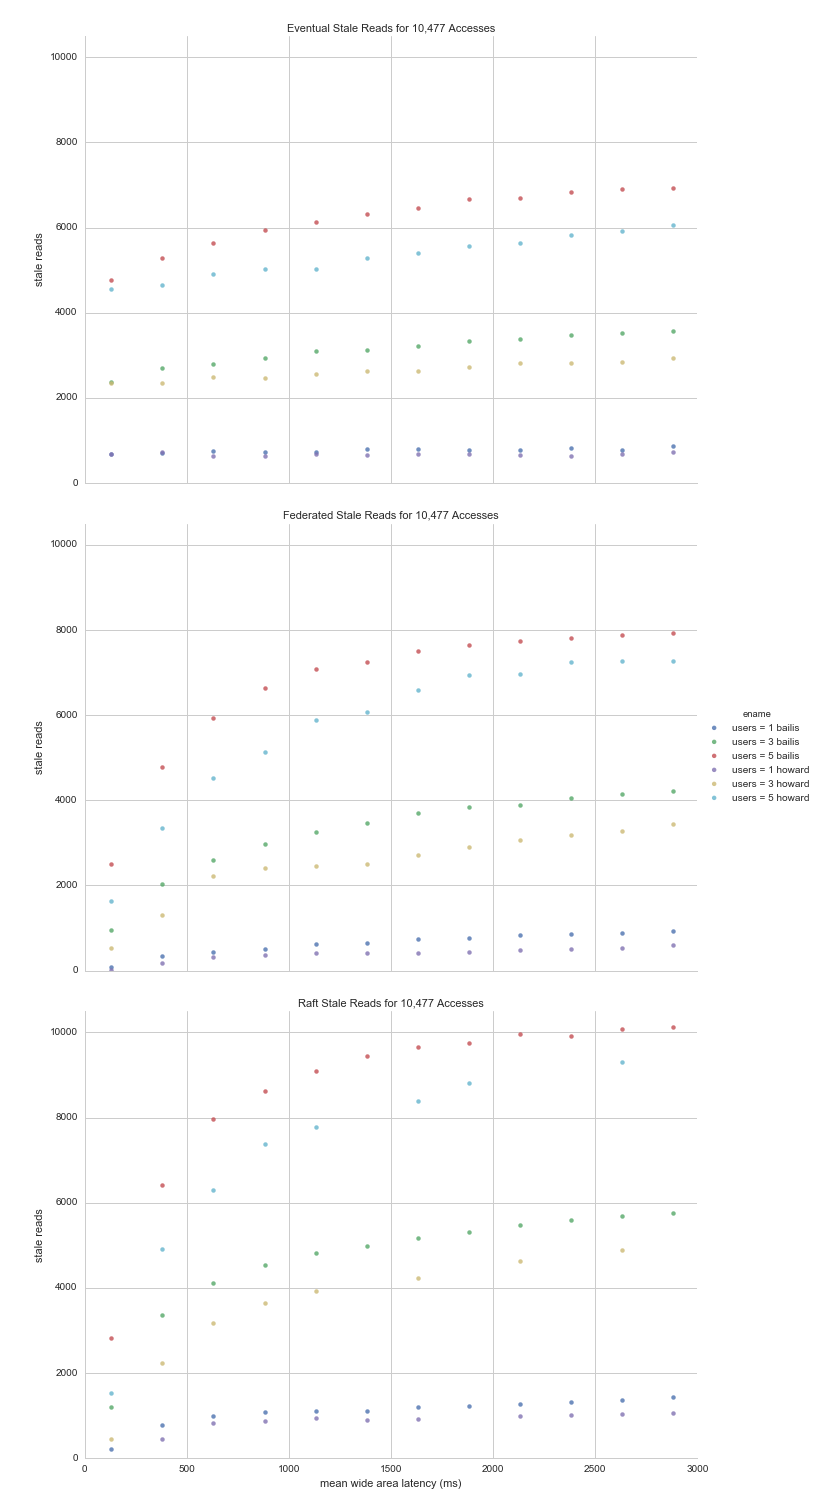
\includegraphics[width=\textwidth]{figures/stale_reads.png}
        \caption{\textsf{Even with READ LATEST, Raft (and consensus implemented sequential consistency) suffers from stale reads. Eventual suffers less, and Federated takes advantage of instantaneous reads on eventual nodes.}}
        \label{fig:stale_reads}
\end{figure}

\begin{figure}[!h]
    \centering
        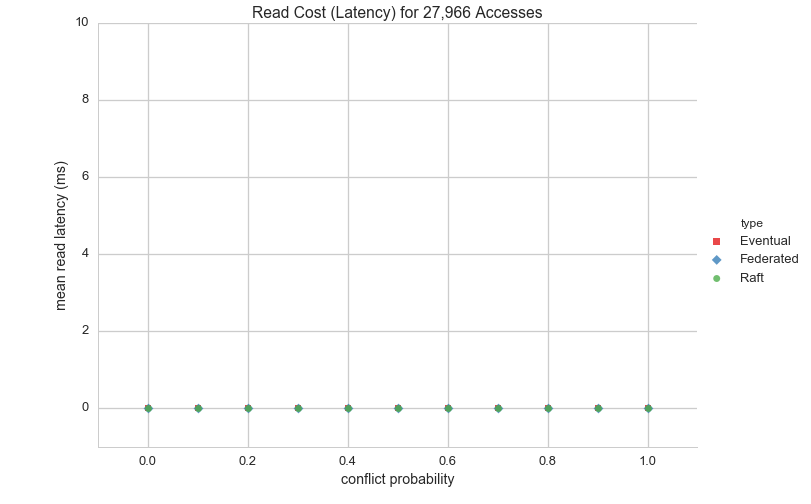
\includegraphics[width=\textwidth]{figures/read_latency.png}
        \caption{\textsf{Question answered: there are no remote reads in this simulation, hence zero read latency.}}
        \label{fig:read_latency}
\end{figure}

\begin{figure}[!h]
    \centering
        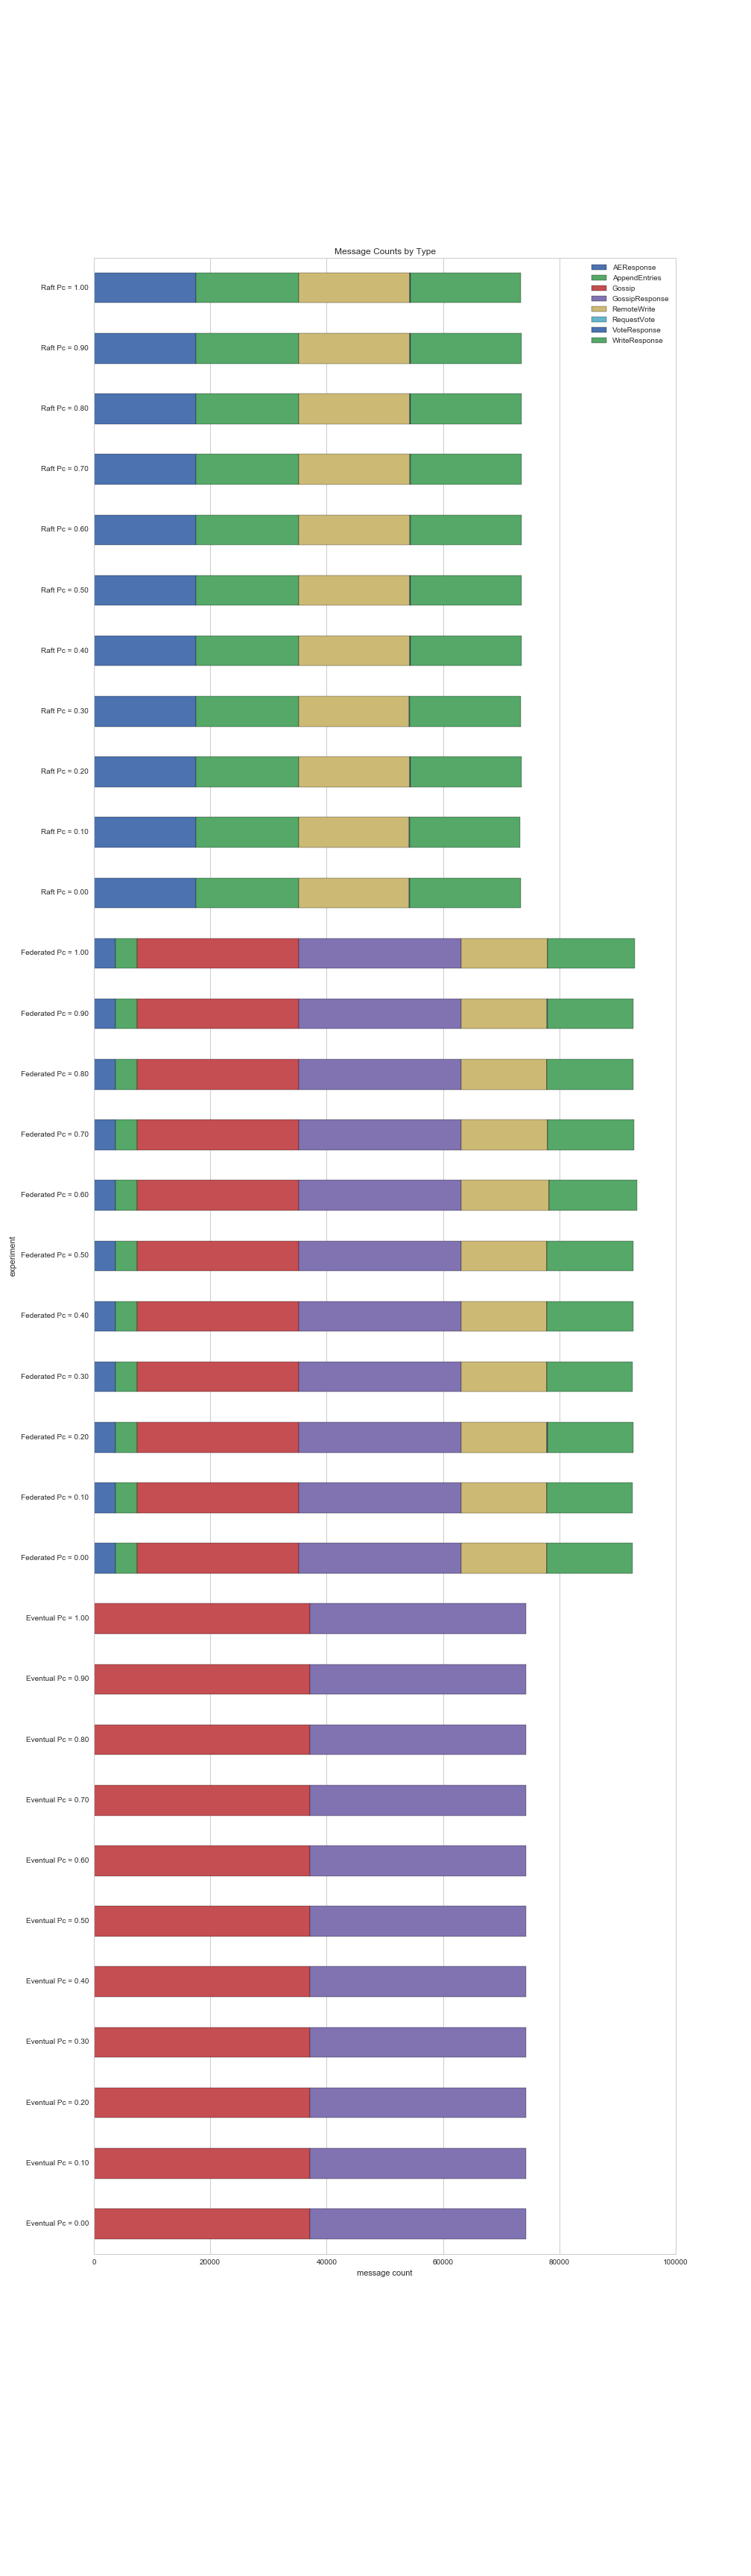
\includegraphics[height=.9\textheight]{figures/message_counts.png}
        \caption{\textsf{See \ref{fig:messages_sent} for more details.}}
        \label{fig:message_counts}
\end{figure}

\begin{figure}[!h]
    \centering
        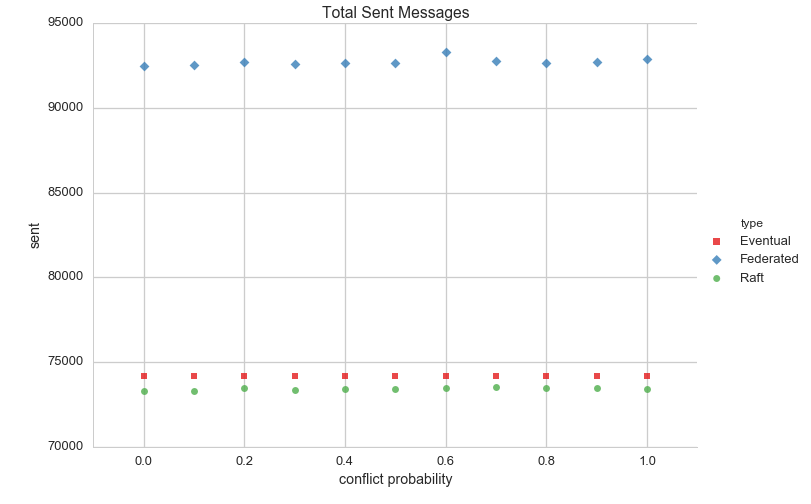
\includegraphics[width=\textwidth]{figures/messages_sent.png}
        \caption{\textsf{So this is the reason that Federated took so much longer to simulate, it has two types of Nodes sending all Eventual messages plus the addition of the consensus messages. Note however that Federated isn't sending twice as many messages; instead it is sending the same number of eventual messages + only a small subset of nodes sending the consensus messages. This is one of the reasons that Hierarchical is needed for the central quorum group; to reduce the number of consensus messages as well as local anti-entropy messages.}}
        \label{fig:messages_sent}
\end{figure}

\begin{figure}[!h]
    \centering
        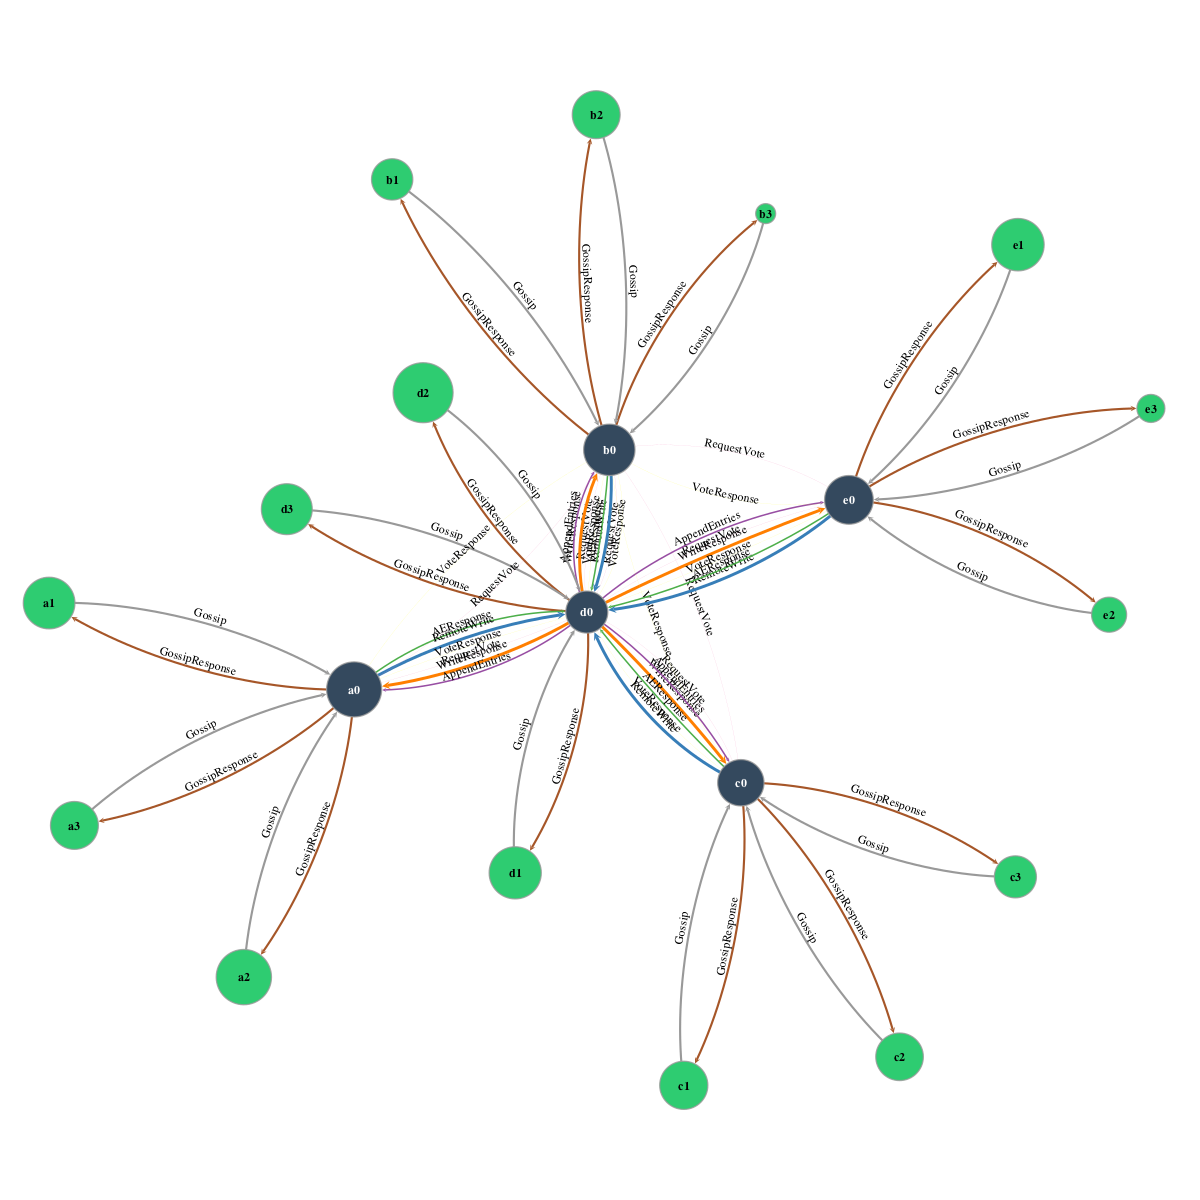
\includegraphics[width=\textwidth]{figures/federated-topology.png}
        \caption{\textsf{Edges define communication by message type (both color and label indicate the message type), message frequency between nodes is indicated by edge thickness. Vertices are colored by their consistency model (Raft and Eventual in Federated). Vertex size indicates the number of \textit{writes} that occurred at that node. Green nodes do send messages across the wide area, but so rarely as to not show up in this figure, this is another parameter that can be tuned and will need to be discussed in the paper.}}
        \label{fig:topology}
\end{figure}


\end{document}
